\documentclass{scrartcl}

\date{\today}

\usepackage[utf8]{inputenc}
\usepackage{graphicx}
\usepackage{hyperref}
\usepackage{subcaption}

\author{Adam Furmańczuk, Nico von Geyso}
\title{
  Technical report \\
  \vspace{0.5cm}
  \small{Spatial Database Project WiSe 2014/2015}
}

\begin{document}

\maketitle

\begin{abstract}
  Topic was to collect historical and forecast weather data. This data then
  should be overlayed on a map. This reports gives you a short introduction
  about the datasets and the implementation. As well there is a step by step
  manual to setup the software locally.
\end{abstract}


\section{Introduction}
The task is to visualize historical and current weather measurements and
forecasts. Part of the assignment is to collect the data itself and overlay that
data with OSM or another map provider.


\section{Data Sources}
\subsection{Historical Data}
Main data source for historical weather measurements is \textit{Deutsche
Wetterdienst}. Measurements for temperature, air pressure and rainfall is
collected from 503 weather stations in Germany. The data is publicly available
through a ftp server:

\begin{center}\url{ftp://ftp.dwd.de/pub/CDC/observations_germany/}\end{center}

It contains data for the past (several month up to years) until today.

\paragraph{Issues}
Weather data from DWD is provided as a collection of geographic points. In order
to produce a nice overlay map, those points need to be transformed to adjacent
polygons. This transformation from points to cells is done through a voronoi
diagram

\subsection{Forecast Data}
Forecast data is provided by the \textit{NOAA\footnote{National Oceanic and
Atmospheric Administration} Global Forecast System}. This dataset gets
calculated through a a global weather forecast model. Data is freely available
for current and past forecasts. The data can be accessed via a ftp server or by
cgi script written in Perl. The format of this data is grib2\footnote{raster
format}.

\paragraph{Issues}
Forecast data from \textit{NOAA GFS} is published in raster format with a $0.5$
degree resolution. To get a nice overlay this groarse resolution needs to be
changed by resizing and interpolating the data. To display the data only
forecasts for Germany are of interest. This is done by intersecting the raster
with a polygon of Germany.



\section{Implementation}
\subsection{Implementation overview}
The implementation is based on Python and a Postgres database with Postgis
extension. Client communication is done through javascript over REST api.
Libraries used are the following:

\begin{description}
  \item [Flask] web framework
  \item [GeoAlchemy] object relational mapper for Postgres/Postgis
  \item [shapely] geospatial library
  \item [Jquery] DOM abstraction
  \item [Leaflet] interactive maps
\end{description}


\subsection{Installation}
The source code along with the installation instruction is available on Github:

\begin{center}
  \url{https://github.com/cholin/fuberlin_spatial_db_project/}
\end{center}

Basically, in order to run the project on the local (linux) machine the
following steps need to be taken:

\paragraph{Database initialization}
Postgres 9.x and Postgis 2.x need to be installed.
\begin{verbatim}
sudo su postgres
createuser -D -P -s -R <username>
createdb -O <username> <database>
\end{verbatim}

\paragraph{Setup}
Source download and dependency installation.
\begin{verbatim}
$ git clone git@github.com:cholin/fuberlin_spatial_db_project.git
$ cd spatial
$ virtualenv2 env
$ . env/bin/activate               # activate virtual environment
$ pip install -r requirements.txt
\end{verbatim}

\textit{HINT}: install numpy via your local distribution package manager.

\paragraph{Configuration} set database credentials

\begin{verbatim}
$ cat config.cfg.dist > config.cfg
$ vim config.cfg                   # set credentials for SQLALCHEMY
\end{verbatim}

\paragraph{Import}
Data import from DWD and NOAA GFS
\begin{verbatim}
$ python2 manage.py resetdb
$ python2 manage.py import_weather                # imports all recent dwd data
$ python2 manage.py import_forecast YYYY-mm-dd    # import forecasts since
                                                  # given date until now
\end{verbatim}


\paragraph{Webserver}
Start the application
\begin{verbatim}
python2 manage.py runserver
\end{verbatim}

The spatial database project is now available on \url{http://localhost:5000}.

\vspace{1cm}

\begin{figure}[h!]
\centering
\begin{subfigure}{.5\textwidth}
  \centering
  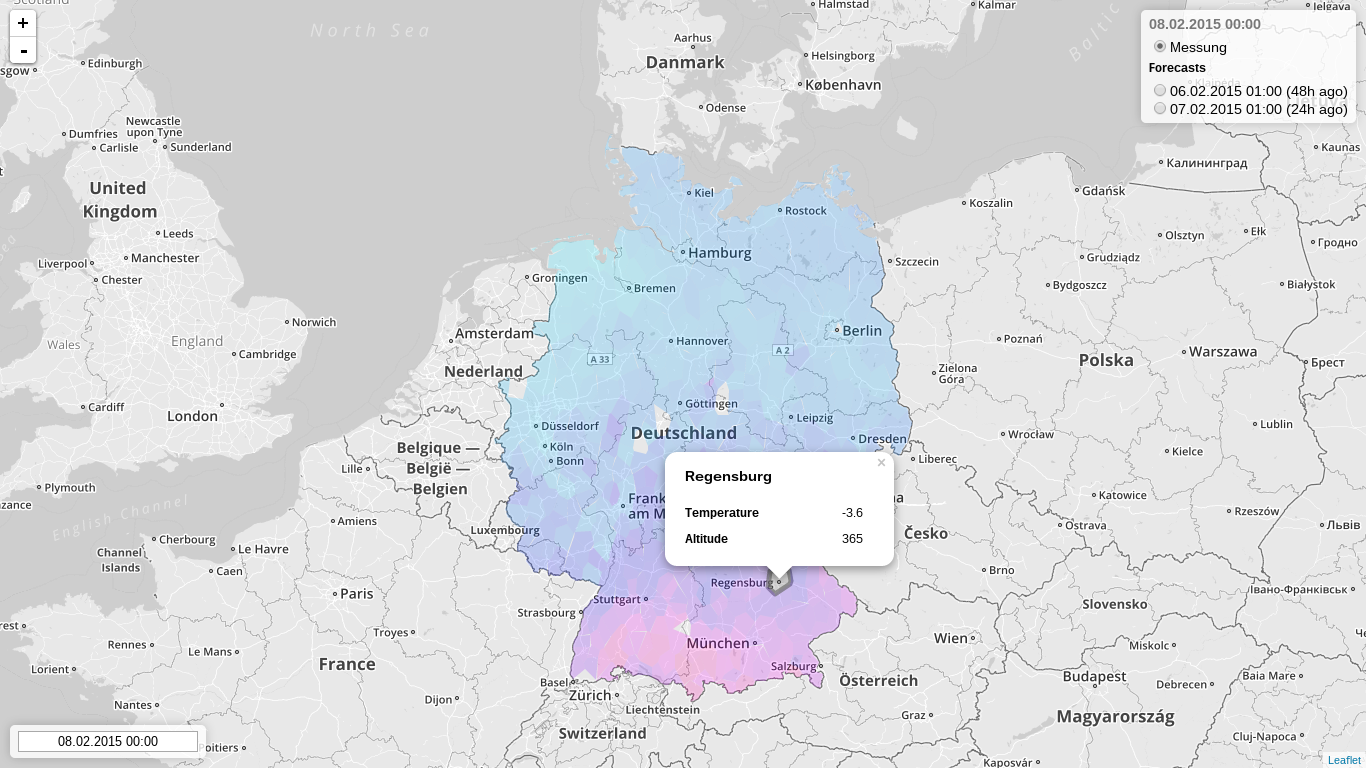
\includegraphics[width=.9\linewidth]{../presentation/images/live_measurement.png}
  \caption{Measurements}
\end{subfigure}%
\begin{subfigure}{.5\textwidth}
  \centering
  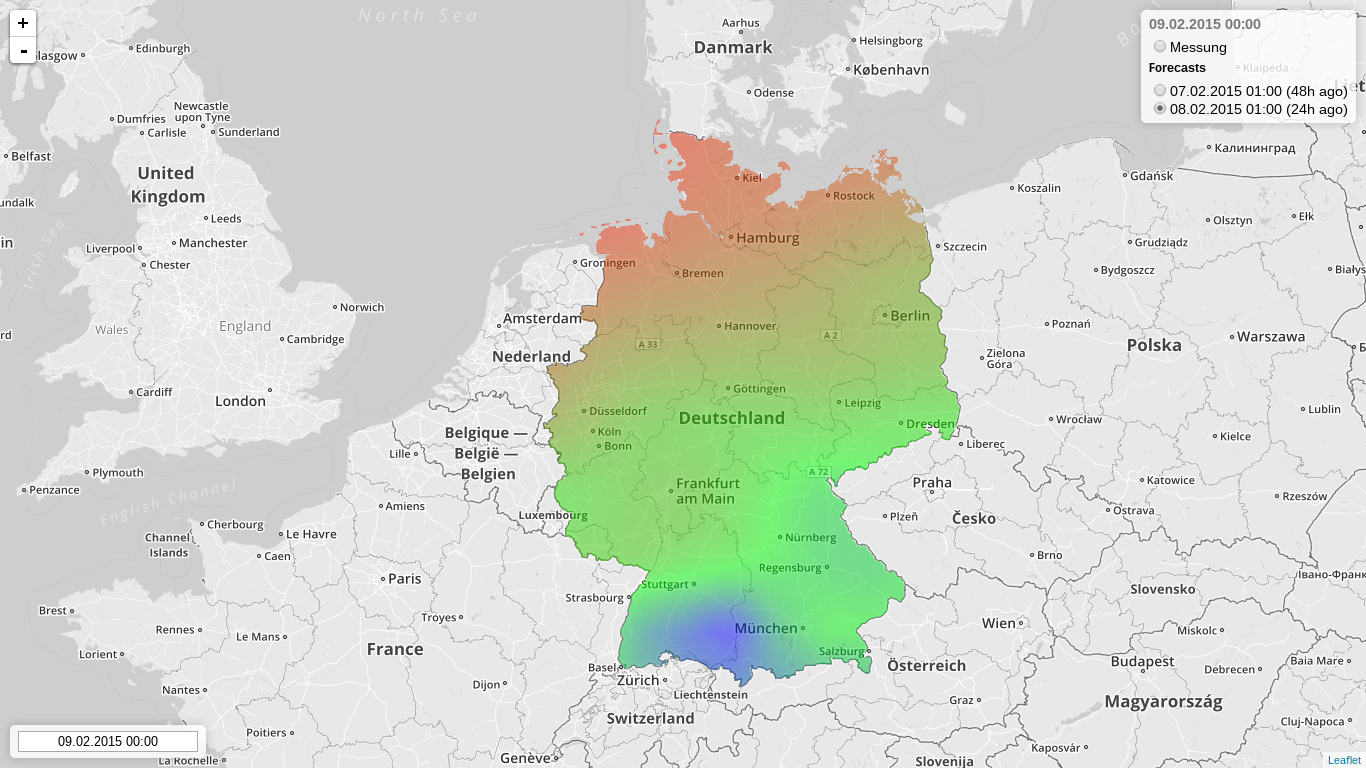
\includegraphics[width=.9\linewidth]{../presentation/images/live_forecast.png}
  \caption{Forecasts}
\end{subfigure}
\caption{Webserver screenshots}
\end{figure}

\section{Issues}
\subsection{Importing weather data}
For \textit{DWD} and \textit{NOAA GFS} there are no existing importers. Therefor
new importers had to be implemented. Furthermore raw weather measurements or
forecast data is not useful at all. This data needs to be transformed and
integrated into the application itself.

\subsection{Documentation}
For data sources nearly no or bad documentation is available. This problem
is most severe on the \textit{NOAA} plattform where variables are not
documented and often results in \textit{try-and-error} methods.

\subsection{Inconsistency}
Another problem was that some data is inconsistent or missing. We chose to leave
them blank if no data is available.

\subsection{Learning curve}
It needs a lot of time to get familiar with different libraries. Often you
realise that a library does not fit your requirements and you have to look for
another one.


\section{Outlook}
This project can be further extended for calculations, datasets and
visualisation.

As for calculations, based on the available data a new forecast system can bei
introduced. 
Futher development effort can be put to include more datasets. Currently, we
use only \textit{DWD} and \textit{NOAA} data sources. include and integrate
more forecast sources. Finally, more work can be put into visualization, in
order to improve usability. 


\section{Summary}
In this project we learned to account for vector and raster data in spatial
databases like Postgres/Postgis. We also learned how to visualize spatial data
using front-end libraries like Leaflet.

\end{document}
